\section{Newton法}
\label{sec:newton-basic}

手里有当前点的梯度和Hessian，下一步应该走到哪里，这样走在什么条件下是对的，又能快到什么程度？

\paragraph{用一个碗代替地形}
设$f:\mathbb{R}^n\to\mathbb{R}$二阶连续可微。站在$\bm{x}^{(t)}$处，把目标在附近作二阶Taylor展开，保留到二次项，得到\term{局部二次模型}（local quadratic model）
\begin{equation}
 m^{(t)}(\bm{d})=f(\bm{x}^{(t)})+(\bm{g}^{(t)})^\top\bm{d}+\frac12\bm{d}^\top\bm{H}^{(t)}\bm{d},
 \label{eq:newton-model}
\end{equation}
其中$\bm{d}$是从当前点出发的位移，$\bm{g}^{(t)}=\nabla f(\bm{x}^{(t)})$，$\bm{H}^{(t)}=\nabla^2f(\bm{x}^{(t)})$。Taylor公式的余项估计可参考\BookChapterRef{chap:multivariate-differentiation}{卷二第20章“多元函数微分”}。

模型和目标在当前点有相同的函数值、斜率和弯曲程度。可以这样想：我们看不到整片地形，只能摸清脚下这一小块的坡度和弯度，于是用一只形状相同的碗去贴合脚下的地面。一阶方法只用一块斜板贴合，斜板告诉我们往哪边倒，却没有底；碗有底，底的位置就是模型给出的下一步。

这个比喻要记住它的限度。碗只在脚下贴合，$\lVert\bm{d}\rVert_2$越大，碗和地形的差别越大。后面几节的大部分工作都是在回答同一个问题：这只碗能信多远。

\paragraph{Newton方程}
当$\bm{H}^{(t)}$正定时，模型是真正的碗，它的底由模型梯度为零确定。对式~\eqref{eq:newton-model}关于$\bm{d}$求梯度并令其为零，得到
\begin{equation}
 \bm{H}^{(t)}\bm{d}^{(t)}=-\bm{g}^{(t)}.
 \label{eq:newton-equation}
\end{equation}
这个线性方程称为\term{Newton方程}（Newton equation），解$\bm{d}^{(t)}$称为\term{Newton方向}（Newton direction）。走满这一步就是\term{Newton法}（Newton's method）：
\begin{equation}
 \bm{x}^{(t+1)}=\bm{x}^{(t)}+\bm{d}^{(t)}.
 \label{eq:newton-update}
\end{equation}
实际计算解方程~\eqref{eq:newton-equation}，不求$(\bm{H}^{(t)})^{-1}$。对称正定方程用Cholesky分解，稠密时约$n^3/3$次运算；分解和回代的做法可参考\BookChapterRef{chap:direct-linear-solvers}{卷二第12章“线性方程的直接求解”}。

一元时方程~\eqref{eq:newton-equation}就是$f''(x)d=-f'(x)$。以$f(x)=e^x-2x$为例，最小点是$x^\star=\ln2\approx0.6931$。这时$f'(x)=e^x-2$，$f''(x)=e^x$，更新为
\[
 x^{(t+1)}=x^{(t)}-\frac{e^{x^{(t)}}-2}{e^{x^{(t)}}}=x^{(t)}-1+2e^{-x^{(t)}}.
\]
从$x^{(0)}=1.5$出发，
\[
 x^{(1)}=1.5-1+2e^{-1.5}\approx0.9463.
\]
一步就把误差从$0.807$降到$0.253$。

\begin{BookInlineFigure}
  \centering
  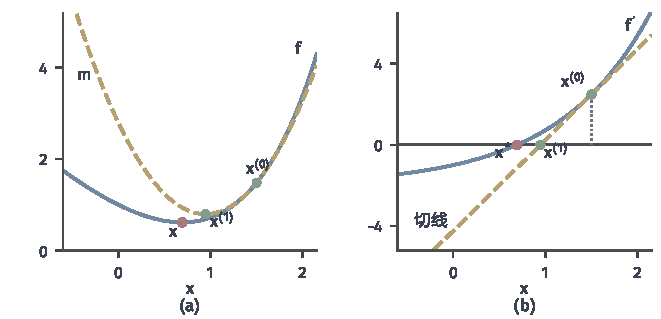
\includegraphics[width=112mm]{figures/05-optimization/02-smooth-optimization/matplotlib/newton-model-1d/figure.pdf}
  \caption{Newton步的两种读法，目标为$f(x)=e^x-2x$，$x^{(0)}=1.5$。(a)蓝线是目标，黄色虚线是在$x^{(0)}$处的二次模型，绿点$x^{(1)}$是模型的极小点，红点是真正的最小点$x^\star$。(b)蓝线是导数$f'$，黄色虚线是它在$x^{(0)}$处的切线，切线与横轴的交点正是同一个$x^{(1)}$。}
  \label{fig:newton-model-1d}
\end{BookInlineFigure}

图~\ref{fig:newton-model-1d}给出同一步的两种读法。图(a)是极小化的读法：用抛物线代替曲线，走到抛物线的底。图(b)是解方程的读法：要找$\nabla f=\bm{0}$的根，就把$\nabla f$在当前点线性化，再求线性函数的根。多元时，线性化$\nabla f(\bm{x}^{(t)}+\bm{d})\approx\bm{g}^{(t)}+\bm{H}^{(t)}\bm{d}$再令其为零，得到的仍是式~\eqref{eq:newton-equation}。

两种读法在正定时一致，但解方程的读法只找驻点，分不清极小点、极大点和鞍点。在$\bm{H}^{(t)}$不正定的地方，两者会分道扬镳，这正是下面要讲的。

\paragraph{贯穿全章的例子}
后面用同一个二元目标检验各种方法：
\begin{equation}
 f(\bm{x})=\frac12(x_1-1)^2+(x_2-x_1^2)^2.
 \label{eq:newton-running-objective}
\end{equation}
两个平方项同时为零当且仅当$\bm{x}=(1,1)$，所以$\bm{x}^\star=(1,1)$，$f^\star=0$。第二项把点拉向抛物线$x_2=x_1^2$，第一项才沿抛物线把点推向解，因此等高线是一条弯曲的山谷。

记$u=x_2-x_1^2$。逐项求导，得到梯度和Hessian：
\begin{equation}
 \nabla f(\bm{x})=\begin{bmatrix}x_1-1-4x_1u\\2u\end{bmatrix},\qquad
 \nabla^2f(\bm{x})=\begin{bmatrix}1-4u+8x_1^2&-4x_1\\-4x_1&2\end{bmatrix}.
 \label{eq:newton-running-derivatives}
\end{equation}
Hessian的右下角元素是$2>0$，行列式为
\[
 \det\nabla^2f(\bm{x})=2(1-4u+8x_1^2)-16x_1^2=2(1-4u).
\]
所以$\nabla^2f(\bm{x})$正定当且仅当$1-4u>0$，也就是点在抛物线$x_2=x_1^2+\tfrac14$的下方。这条抛物线上方的区域里Hessian不定，下面的图都用红色浅底标出。

这个例子的Newton方程能手解。由第二行得$d_2=-u+2x_1d_1$，代入第一行，含$8x_1^2$的项互相抵消，只剩$(1-4u)d_1=1-x_1$。于是，当$1-4u\neq0$时，
\begin{equation}
 d_1=\frac{1-x_1}{1-4u},\qquad d_2=-u+2x_1d_1.
 \label{eq:newton-running-direction}
\end{equation}

图~\ref{fig:newton-model-trust}比较模型和目标。在$(\tfrac12,0)$附近，模型的黄色椭圆和目标的蓝色等高线相当接近，模型的底$(\tfrac34,\tfrac12)$确实比出发点低。在$(-1,\tfrac65)$处情况完全不同：Hessian的两个特征值约为$10.16$和$0.039$，模型沿一个方向几乎是平的，由式~\eqref{eq:newton-running-direction}算出模型的底远在$(9,-19)$。

\begin{BookInlineFigure}
  \centering
  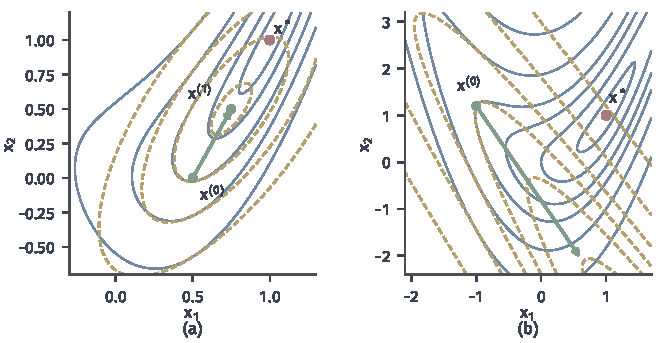
\includegraphics[width=112mm]{figures/05-optimization/02-smooth-optimization/matplotlib/newton-model-trust/figure.pdf}
  \caption{式~\eqref{eq:newton-running-objective}的等高线（蓝）与局部模型的等高线（黄色虚线）。(a)在$(\tfrac12,0)$处模型贴合良好，绿色箭头是Newton步，它的终点$\bm{x}^{(1)}$是模型的极小点。(b)在$(-1,\tfrac65)$处模型是一条几乎平直的长沟，绿色箭头按实际长度的$0.16$倍绘制，模型极小点$(9,-19)$在图外。两图中红点都是$\bm{x}^\star$。}
  \label{fig:newton-model-trust}
\end{BookInlineFigure}

\paragraph{可逆与正定各管什么}
方程~\eqref{eq:newton-equation}有唯一解只要求$\bm{H}^{(t)}$可逆；这个解是模型的极小点、并且指向下坡，要求的是正定。下面的结论把这两件事分开。

\begin{lemma}[正定曲率下的Newton方向]
\label{lem:newton-spd-direction}
设$\bm{H}^{(t)}\succ\bm{0}$，$\bm{g}^{(t)}\neq\bm{0}$。则$\bm{d}^{(t)}=-(\bm{H}^{(t)})^{-1}\bm{g}^{(t)}$是模型~\eqref{eq:newton-model}的唯一极小点，且满足
\begin{equation}
 (\bm{g}^{(t)})^\top\bm{d}^{(t)}=-(\bm{g}^{(t)})^\top(\bm{H}^{(t)})^{-1}\bm{g}^{(t)}<0.
 \label{eq:newton-descent}
\end{equation}
\end{lemma}

\begin{proof}
省略上标。任取位移$\bm{d}$，写成$\bm{d}=\bm{d}^{(t)}+\bm{w}$代入模型。一次项中用$\bm{g}=-\bm{H}\bm{d}^{(t)}$，含$\bm{w}$的一次项互相抵消，得到
\[
 m(\bm{d})=m(\bm{d}^{(t)})+\frac12\bm{w}^\top\bm{H}\bm{w}.
\]
$\bm{H}$正定，所以$\bm{w}\neq\bm{0}$时第二项严格为正，$\bm{d}^{(t)}$是唯一极小点。

下降性由定义代入得到。$\bm{H}$正定时$\bm{H}^{-1}$也正定，而$\bm{g}\neq\bm{0}$，于是二次型$\bm{g}^\top\bm{H}^{-1}\bm{g}$严格为正。
\end{proof}

图~\ref{fig:newton-curvature-cases}用三种曲率说明不正定时会发生什么。图(a)的$\bm{H}$正定，等高线是椭圆，方程的解是碗底。图(b)的$\bm{H}$可逆但不定，方程仍有唯一解，那个点却是马鞍的中心，模型沿某些方向可以无限下降，“走到模型的底”这句话失去了意义。图(c)的$\bm{H}$奇异，且$\bm{g}$不在它的值域内，方程无解，模型沿平坦方向一直倾斜。

\begin{BookInlineFigure}
  \centering
  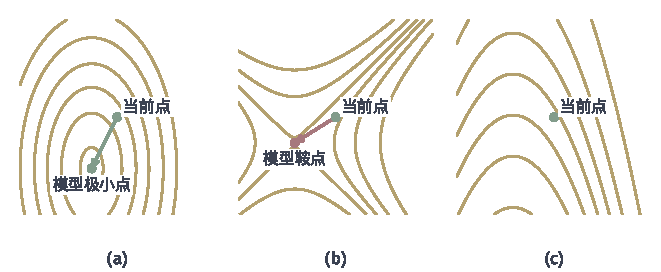
\includegraphics[width=112mm]{figures/05-optimization/02-smooth-optimization/matplotlib/newton-curvature-cases/figure.pdf}
  \caption{三种曲率下的局部模型，黄线为$m(\bm{d})$的等高线，绿色圆点是当前点。(a)$\bm{H}=\operatorname{diag}(2,0.6)$正定，Newton方程的解是模型的极小点。(b)$\bm{H}=\operatorname{diag}(1,-1)$不定，方程的解是模型的鞍点，用红色标出。(c)$\bm{H}=\operatorname{diag}(1,0)$奇异，$\bm{g}=(0.8,0.5)$不在值域内，方程无解。}
  \label{fig:newton-curvature-cases}
\end{BookInlineFigure}

在例子中可以看到“不定”的具体后果。取$\bm{x}=(0,\tfrac12)$，此时$u=\tfrac12$，$1-4u=-1<0$。由式~\eqref{eq:newton-running-derivatives}，
\[
 \bm{g}=\begin{bmatrix}-1\\1\end{bmatrix},\qquad
 \bm{H}=\begin{bmatrix}-1&0\\0&2\end{bmatrix}.
\]
由式~\eqref{eq:newton-running-direction}，Newton方向是$\bm{d}=(-1,-\tfrac12)$。方向导数为
\[
 \bm{g}^\top\bm{d}=1-\tfrac12=\tfrac12>0,
\]
所以这是一个上坡方向。走满一步到$(-1,0)$，目标从$0.75$升到$3$。

下表把三种情形并排。

\begin{BookInlineTable}
  \centering
  \begin{tabular}{@{}llll@{}}
    \toprule
    $\bm{H}^{(t)}$ & 方程~\eqref{eq:newton-equation} & 解的含义 & 方向 \\
    \midrule
    正定 & 唯一解 & 模型的唯一极小点 & 下降 \\
    可逆但不定 & 唯一解 & 模型的鞍点 & 可升可降 \\
    奇异 & 无解或无穷多解 & 无极小点或极小点不唯一 & 须另行处理 \\
    \bottomrule
  \end{tabular}
  \caption{曲率矩阵的性质与Newton方程的解。可逆只回答方程能否解，正定才回答解是否有用。}
  \label{tab:newton-curvature-cases}
\end{BookInlineTable}

\paragraph{不受坐标伸缩的影响}
Newton方向还有一个梯度方向没有的性质。第~\ref{chap:first-order-methods}章的方法在病态目标上吃亏，原因是步子的大小和各方向的弯度不匹配。Newton方向把弯度算进去了，因此和坐标的单位无关，就像一段路程不会因为改用千米记录而变长。

设$\bm{A}$是可逆矩阵，令$\bm{y}=\bm{A}\bm{x}$，$\tilde f(\bm{y})=f(\bm{A}^{-1}\bm{y})$。由链式法则，新坐标下的梯度和Hessian是
\[
 \nabla\tilde f=\bm{A}^{-\top}\bm{g},\qquad \nabla^2\tilde f=\bm{A}^{-\top}\bm{H}\bm{A}^{-1}.
\]
代入Newton方程，$\bm{A}^{-\top}$互相抵消，新坐标下的方向是
\[
 \tilde{\bm{d}}=-\bm{A}\bm{H}^{-1}\bm{A}^{\top}\bm{A}^{-\top}\bm{g}=\bm{A}\bm{d}.
\]
所以$\tilde{\bm{d}}$恰好是原方向$\bm{d}$在新坐标下的样子，整条迭代序列只是被$\bm{A}$映到了新坐标，这称为\term{仿射不变性}（affine invariance）。

负梯度方向不同。新坐标下它是$-\bm{A}^{-\top}\bm{g}$，而把原方向$-\bm{g}$映过去是$-\bm{A}\bm{g}$，两者只在$\bm{A}$为正交矩阵的倍数时平行。

图~\ref{fig:newton-affine}以$f(\bm{x})=\tfrac12(x_1^2+25x_2^2)$为例，条件数是$25$。Newton方向$\bm{d}=-\bm{H}^{-1}\bm{H}\bm{x}=-\bm{x}$，从任何起点都一步到达最小点，这对任意正定二次目标都成立。使用精确线搜索的梯度下降在原坐标下往复前进；换坐标$y_2=5x_2$后，等高线成了圆，两种方法才走同一条路。

\begin{BookInlineFigure}
  \centering
  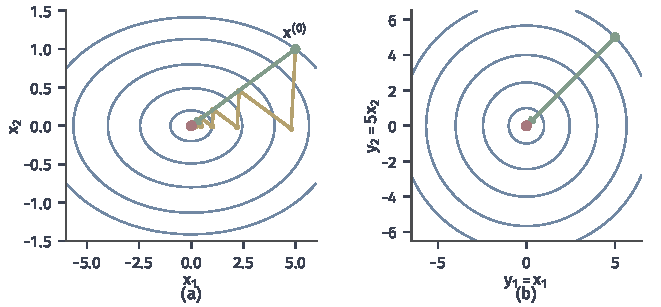
\includegraphics[width=112mm]{figures/05-optimization/02-smooth-optimization/matplotlib/newton-affine/figure.pdf}
  \caption{坐标变换对两种方向的影响，目标$\tfrac12(x_1^2+25x_2^2)$。(a)原坐标，从$(5,1)$出发，黄色折线是精确线搜索的梯度下降，绿色箭头是Newton步，红点是最小点。(b)取$y_2=5x_2$后等高线为圆，负梯度方向和Newton方向重合。Newton步在两张图中是同一步，只是用不同坐标表示。}
  \label{fig:newton-affine}
\end{BookInlineFigure}

仿射不变性说的是精确算术下的迭代。实际解方程时，$\bm{H}^{(t)}$的条件数仍然影响舍入误差，只是它不再决定迭代步数。

\paragraph{计算过程}
Newton法的公式已经由式~\eqref{eq:newton-equation}、\eqref{eq:newton-update}给出。下面用目标~\eqref{eq:newton-running-objective}从$(\tfrac12,0)$出发走一遍。这一节假定每个迭代点的Hessian都正定；不正定的情形由第~\ref{sec:newton-modified}节处理。

\needspace{6\baselineskip}
\paragraph{变量}
\begin{itemize}
 \item $\bm{x}\in\mathbb{R}^n$：当前点$\bm{x}^{(t)}$，在原处更新。
 \item $\bm{g}\in\mathbb{R}^n$：当前梯度。
 \item $\bm{H}\in\mathbb{R}^{n\times n}$：当前Hessian，对称。
 \item $\bm{L}\in\mathbb{R}^{n\times n}$：下三角矩阵，$\bm{H}$的Cholesky因子。
 \item $\bm{d}\in\mathbb{R}^n$：Newton方向。
 \item $\varepsilon>0$：梯度容差。
\end{itemize}

\paragraph{初始化}
选定初始点$\bm{x}^{(0)}$和容差$\varepsilon$，令$t=0$。例中初始点和容差为
\[
 \bm{x}^{(0)}=\bigl(\tfrac12,0\bigr),\qquad \varepsilon=10^{-6}.
\]

\needspace{6\baselineskip}
\paragraph{每轮更新}
在第$t$轮：
\begin{enumerate}
 \item \textbf{读取导数并检查停止。}计算$\bm{g}^{(t)}$和$\bm{H}^{(t)}$。若$\lVert\bm{g}^{(t)}\rVert_2\leq\varepsilon$，输出$\bm{x}^{(t)}$并结束。

 例中第一轮$u=-\tfrac14$，由式~\eqref{eq:newton-running-derivatives}，
 \[
  \bm{g}^{(0)}=\begin{bmatrix}0\\-\tfrac12\end{bmatrix},\qquad
  \bm{H}^{(0)}=\begin{bmatrix}4&-2\\-2&2\end{bmatrix}.
 \]

 \item \textbf{分解。}计算Cholesky分解$\bm{H}^{(t)}=\bm{L}\bm{L}^\top$。

 例中第一轮
 \[
  \bm{L}=\begin{bmatrix}2&0\\-1&1\end{bmatrix}.
 \]

 \item \textbf{回代求方向。}先由前代解$\bm{L}\bm{y}=-\bm{g}^{(t)}$，再由回代解$\bm{L}^\top\bm{d}^{(t)}=\bm{y}$。

 例中第一轮的中间向量和方向分别是
 \[
  \bm{y}=\begin{bmatrix}0\\\tfrac12\end{bmatrix},\qquad
  \bm{d}^{(0)}=\begin{bmatrix}\tfrac14\\\tfrac12\end{bmatrix}.
 \]

 \item \textbf{更新。}按式~\eqref{eq:newton-update}走到下一点，令$t\leftarrow t+1$。

 例中第一轮到达$\bm{x}^{(1)}=(\tfrac34,\tfrac12)$，目标从$\tfrac3{16}$降到$\tfrac9{256}\approx0.0352$。

 第二轮$u=\tfrac12-\tfrac9{16}=-\tfrac1{16}$。这时用手解直接套式~\eqref{eq:newton-running-direction}更快：
 \[
  d_1=\frac{1/4}{1+1/4}=\frac15,\qquad
  d_2=\frac1{16}+\frac32\cdot\frac15=0.3625.
 \]
 于是$\bm{x}^{(2)}=(0.95,0.8625)$，目标降到$0.00285$。
\end{enumerate}

各轮结果列在表~\ref{tab:newton-pure-run}中。第$5$轮梯度范数已低于容差，迭代结束，最终得到$\bm{x}^{(5)}\approx(1,1)$，与解的距离约$2.4\times10^{-8}$。图~\ref{fig:newton-path}画出了前几步的路径。

\begin{BookInlineTable}
  \centering
  \small
  \begin{tabular}{@{}cccccc@{}}
    \toprule
    $t$ & $\bm{x}^{(t)}$ & $f$ & $\lVert\bm{g}^{(t)}\rVert_2$ & $\bm{d}^{(t)}$ & $\lVert\bm{x}^{(t)}-\bm{x}^\star\rVert_2$ \\
    \midrule
    $0$ & $(0.5,0)$ & $0.1875$ & $0.5$ & $(0.25,0.5)$ & $1.118$ \\
    $1$ & $(0.75,0.5)$ & $0.03516$ & $0.1398$ & $(0.2,0.3625)$ & $0.5590$ \\
    $2$ & $(0.95,0.8625)$ & $2.85\mathrm{e}{-3}$ & $0.1296$ & $(0.0431,0.1219)$ & $0.1463$ \\
    $3$ & $(0.9931,0.9844)$ & $2.72\mathrm{e}{-5}$ & $3.75\mathrm{e}{-3}$ & $(0.0068,0.0155)$ & $0.01706$ \\
    $4$ & $(0.99995,0.99985)$ & $3.49\mathrm{e}{-9}$ & $1.66\mathrm{e}{-4}$ & $(5\mathrm{e}{-5},1.5\mathrm{e}{-4})$ & $1.57\mathrm{e}{-4}$ \\
    $5$ & $(1.0000,1.0000)$ & $5.2\mathrm{e}{-17}$ & $5.2\mathrm{e}{-9}$ & 停止 & $2.4\mathrm{e}{-8}$ \\
    \bottomrule
  \end{tabular}
  \caption{Newton法在目标~\eqref{eq:newton-running-objective}上从$(\tfrac12,0)$出发的迭代。第$3$行以后，误差每步大约平方一次。}
  \label{tab:newton-pure-run}
\end{BookInlineTable}

\begin{BookInlineFigure}
  \centering
  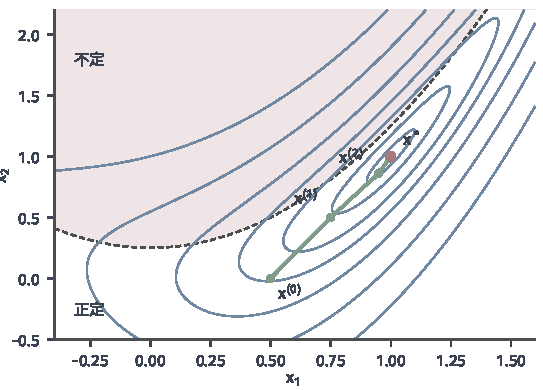
\includegraphics[width=92mm]{figures/05-optimization/02-smooth-optimization/matplotlib/newton-path/figure.pdf}
  \caption{Newton法的迭代路径（绿）。蓝线是目标~\eqref{eq:newton-running-objective}的等高线，红色浅底是Hessian不定的区域，深灰色虚线是它的边界$x_2=x_1^2+\tfrac14$，红点是解。起点$(\tfrac12,0)$在正定区域内，路径紧贴山谷前进，始终没有进入浅底区域。}
  \label{fig:newton-path}
\end{BookInlineFigure}

路径始终在正定区域内，这一点在本例中可以验证。整步之后的$u$值为
\[
 u^{+}=(x_2+d_2)-(x_1+d_1)^2=u+d_2-2x_1d_1-d_1^2.
\]
代入式~\eqref{eq:newton-running-direction}的$d_2$，前三项相消，得到
\[
 u^{+}=-d_1^2\leq0.
\]
因此任意一个完整Newton步之后都有$1-4u^+\geq1>0$。这是此目标特有的结构，一般目标没有这样的保证。

\paragraph{局部二次收敛}
表~\ref{tab:newton-pure-run}最后几行显示，误差接近解时每步大约平方一次。下面说明这种现象来自哪里。先从直观上看：在解附近，目标和它的二次模型只差三阶小量；二次模型的极小点又恰好由Newton步算出，所以Newton步的误差只由这个三阶差决定，比一阶方法“每步打一个固定折扣”好得多。

称一列点\term{二次收敛}（quadratic convergence）到$\bm{x}^\star$，如果存在常数$C$，使充分大的$t$都满足
\begin{equation}
 \lVert\bm{x}^{(t+1)}-\bm{x}^\star\rVert_2\leq C\lVert\bm{x}^{(t)}-\bm{x}^\star\rVert_2^2.
 \label{eq:newton-quadratic-definition}
\end{equation}
定理需要在解附近控制Hessian，记$\mu$为解处Hessian的最小特征值，$M$为Hessian的Lipschitz常数。

\begin{theorem}[Newton法的局部二次收敛]
\label{thm:newton-local}
设$f$在以$\bm{x}^\star$为中心、半径为$r$的开球$\bm{B}$上二阶连续可微，$\nabla f(\bm{x}^\star)=\bm{0}$，$\nabla^2f(\bm{x}^\star)\succeq\mu\bm{I}$，其中$\mu>0$，并且对$\bm{x},\bm{y}\in\bm{B}$有
\begin{equation}
 \lVert\nabla^2f(\bm{x})-\nabla^2f(\bm{y})\rVert_2\leq M\lVert\bm{x}-\bm{y}\rVert_2.
 \label{eq:newton-hessian-lipschitz}
\end{equation}
记$\rho=\min\{r,\ \mu/(2M)\}$。若$\lVert\bm{x}^{(t)}-\bm{x}^\star\rVert_2<\rho$，则$\bm{H}^{(t)}\succeq\tfrac\mu2\bm{I}$，Newton步有定义，且
\begin{equation}
 \lVert\bm{x}^{(t+1)}-\bm{x}^\star\rVert_2\leq\frac{M}{\mu}\lVert\bm{x}^{(t)}-\bm{x}^\star\rVert_2^2.
 \label{eq:newton-quadratic-bound}
\end{equation}
因此，只要$\lVert\bm{x}^{(0)}-\bm{x}^\star\rVert_2<\rho$，所有迭代点都留在半径$\rho$的球内，并且
\begin{equation}
 \frac{M}{\mu}\lVert\bm{x}^{(t)}-\bm{x}^\star\rVert_2\leq\Bigl(\frac12\Bigr)^{2^t}.
 \label{eq:newton-doubly-exponential}
\end{equation}
\end{theorem}

\begin{proof}
记$\bm{e}=\bm{x}^{(t)}-\bm{x}^\star$，$\bm{H}=\bm{H}^{(t)}$，并设$\lVert\bm{e}\rVert_2<\rho$。

第一步说明$\bm{H}$的逆有界。由式~\eqref{eq:newton-hessian-lipschitz}，
\[
 \lVert\bm{H}-\nabla^2f(\bm{x}^\star)\rVert_2\leq M\lVert\bm{e}\rVert_2\leq\frac\mu2.
\]
对称矩阵的特征值受扰动量控制，所以$\lambda_{\min}(\bm{H})\geq\mu-\mu/2$，即
\[
 \bm{H}\succeq\frac\mu2\bm{I},\qquad \lVert\bm{H}^{-1}\rVert_2\leq\frac2\mu.
\]

第二步写出误差的递推。由$\nabla f(\bm{x}^\star)=\bm{0}$，沿线段积分，
\[
 \bm{g}^{(t)}=\int_0^1\nabla^2f(\bm{x}^\star+s\bm{e})\bm{e}\,\mathrm{d}s.
\]
Newton步之后的误差是$\bm{e}-\bm{H}^{-1}\bm{g}^{(t)}$。把$\bm{e}$写成$\bm{H}^{-1}\bm{H}\bm{e}$并合并，得到
\[
 \bm{x}^{(t+1)}-\bm{x}^\star=\bm{H}^{-1}\int_0^1\bigl(\bm{H}-\nabla^2f(\bm{x}^\star+s\bm{e})\bigr)\bm{e}\,\mathrm{d}s.
\]

第三步估计积分。点$\bm{x}^{(t)}$与$\bm{x}^\star+s\bm{e}$相距$(1-s)\lVert\bm{e}\rVert_2$，由式~\eqref{eq:newton-hessian-lipschitz}，
\[
 \Bigl\lVert\int_0^1\bigl(\bm{H}-\nabla^2f(\bm{x}^\star+s\bm{e})\bigr)\bm{e}\,\mathrm{d}s\Bigr\rVert_2
 \leq\int_0^1M(1-s)\lVert\bm{e}\rVert_2^2\,\mathrm{d}s=\frac M2\lVert\bm{e}\rVert_2^2.
\]
与第一步的$2/\mu$相乘，即得式~\eqref{eq:newton-quadratic-bound}。

最后讨论序列。记
\[
 a_t=\frac M\mu\lVert\bm{x}^{(t)}-\bm{x}^\star\rVert_2,
\]
式~\eqref{eq:newton-quadratic-bound}写成$a_{t+1}\leq a_t^2$。由初始距离小于$\rho\leq\mu/(2M)$得$a_0<\tfrac12$。于是误差每步至少减半，迭代点不离开球，归纳得$a_t\leq a_0^{2^t}\leq(\tfrac12)^{2^t}$。
\end{proof}

式~\eqref{eq:newton-doubly-exponential}说明，进入这个邻域后，有效数字大约每步翻倍。回到$f(x)=e^x-2x$，从$1.5$出发的误差依次是
\[
 0.807,\quad 0.253,\quad 0.0295,\quad 4.31\times10^{-4},\quad 9.27\times10^{-8},\quad 4.33\times10^{-15}.
\]
相邻两步的比值$e^{(t+1)}/(e^{(t)})^2$依次约为
\[
 0.39,\quad 0.46,\quad 0.50,\quad 0.50,\quad 0.50,
\]
趋于$f'''(x^\star)/(2f''(x^\star))=\tfrac12$。

对主例~\eqref{eq:newton-running-objective}，解处Hessian的特征值约为$0.185$和$10.8$，所以$\mu\approx0.185$；在解附近数值估计$M\approx25$，定理保证的半径$\mu/(2M)$只有约$0.0037$。表~\ref{tab:newton-pure-run}的迭代却从距离$1.1$处就进展顺利。定理给出的是充分条件，半径通常十分保守；它的价值在于说明快速收敛的机制和所需的条件。

图~\ref{fig:newton-order}(a)比较了同一起点上的Newton法和使用回溯线搜索的梯度下降，后者的步长规则由下一节的式~\eqref{eq:newton-armijo}规定。解处的条件数约为$58$，梯度下降要$245$步才能把梯度范数降到$10^{-6}$，Newton法用了$5$步。

\begin{BookInlineFigure}
  \centering
  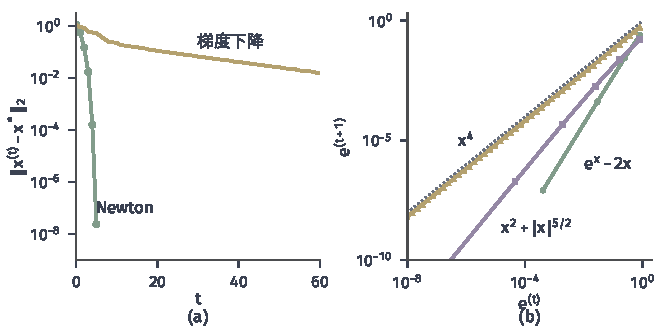
\includegraphics[width=112mm]{figures/05-optimization/02-smooth-optimization/matplotlib/newton-order/figure.pdf}
  \caption{收敛阶的比较。(a)目标~\eqref{eq:newton-running-objective}上从$(\tfrac12,0)$出发的距离误差，绿线为Newton法，黄线为回溯梯度下降。(b)双对数坐标下相邻两步一维误差的关系：绿线$e^x-2x$斜率约为$2$，紫线$x^2+\lvert x\rvert^{5/2}$斜率约为$1.5$，黄线$x^4$斜率为$1$且接近灰色虚线$e^{(t+1)}=e^{(t)}$。}
  \label{fig:newton-order}
\end{BookInlineFigure}

\paragraph{三个条件的作用}
定理有三个条件：解处Hessian正定、Hessian Lipschitz连续、初始点足够近。逐一去掉，可以看到结论怎样变弱。

去掉解处正定，看$f(x)=x^4$。解是$0$，但$f''(0)=0$，这是退化的极小点。Newton更新为
\[
 x^{(t+1)}=x^{(t)}-\frac{4(x^{(t)})^3}{12(x^{(t)})^2}=\frac23x^{(t)}.
\]
收敛只是线性的，误差每步乘以固定的$\tfrac23$。式~\eqref{eq:newton-quadratic-bound}中的$M/\mu$此时为无穷大，模型的底沿平坦方向已不再贴近真解。

去掉Hessian的Lipschitz连续，看$f(x)=x^2+\lvert x\rvert^{5/2}$。它的解是$0$，$f''(0)=2$，但$f''$在$0$处只是$\tfrac12$阶Hölder连续。对$x>0$，
\[
 f'(x)=2x+\tfrac52x^{3/2},\qquad f''(x)=2+\tfrac{15}4x^{1/2}.
\]
代入Newton更新并通分，分子中的一次项抵消，得到
\[
 x^{(t+1)}=\frac{\frac54(x^{(t)})^{3/2}}{2+\frac{15}4(x^{(t)})^{1/2}}\approx\frac58(x^{(t)})^{3/2}.
\]
误差的阶从$2$降为$\tfrac32$，仍快于线性，但不再是二次。图~\ref{fig:newton-order}(b)中三条线的斜率正是收敛阶。

去掉初始点足够近，看严格凸函数$\varphi(x)=\sqrt{1+x^2}$。求导得
\[
 \varphi'(x)=\frac{x}{\sqrt{1+x^2}},\qquad \varphi''(x)=(1+x^2)^{-3/2}.
\]
代入Newton更新，得到极简的递推
\begin{equation}
 x^{(t+1)}=x^{(t)}-x^{(t)}\bigl(1+(x^{(t)})^2\bigr)=-(x^{(t)})^3.
 \label{eq:newton-cubic-map}
\end{equation}
$\lvert x^{(0)}\rvert<1$时迭代收敛，$\lvert x^{(0)}\rvert=1$时在$\pm1$之间来回跳，$\lvert x^{(0)}\rvert>1$时发散。图~\ref{fig:newton-basin}(a)说明了原因：$x$很大时函数几乎是直线，曲率很小，模型的底在非常远的地方。这个函数处处解析、处处严格凸，Newton法照样发散，所以局部定理中的“足够近”不能省略。

\begin{BookInlineFigure}
  \centering
  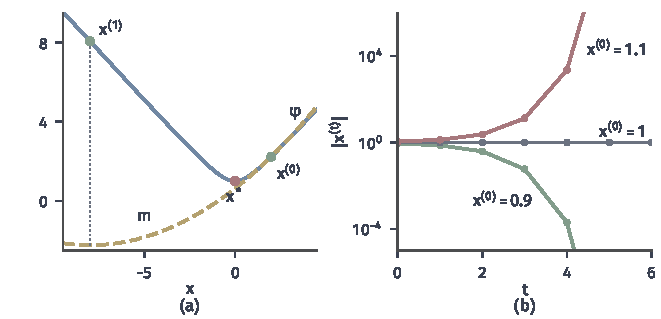
\includegraphics[width=112mm]{figures/05-optimization/02-smooth-optimization/matplotlib/newton-basin/figure.pdf}
  \caption{严格凸函数$\varphi(x)=\sqrt{1+x^2}$上Newton法的局部性。(a)蓝线是$\varphi$，黄色虚线是$x^{(0)}=2$处的二次模型，模型的底在$x=-8$，绿点标出实际到达的新点，$\varphi$反而升高。(b)递推$x^{(t+1)}=-(x^{(t)})^3$的三条轨迹，纵轴为绝对值，初值分别为$0.9$（绿）、$1$（灰）、$1.1$（红）。}
  \label{fig:newton-basin}
\end{BookInlineFigure}
